\documentclass{standalone}

\usepackage{tikz}
\usepackage{graphicx}
\pagestyle{empty}

% INT_AY20_MP1_L13-Fig05-Find_missing_angle_ans.png

\begin{document}
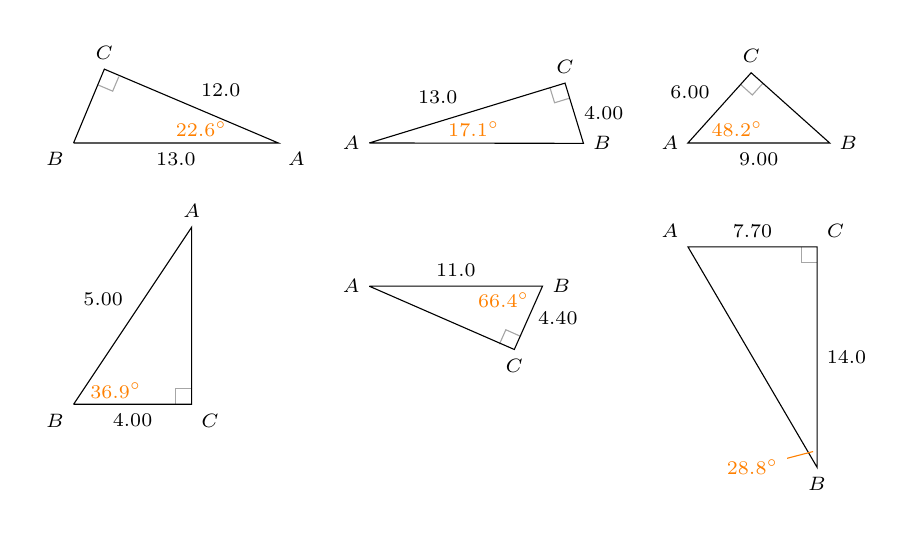
\begin{tikzpicture}[font = \scriptsize]

\matrix[column sep = 0.25 cm, row sep = 0.25 cm, ampersand replacement = \&]{

	\draw [gray!70] (67 : 0.8) -- ++ (-23 : 0.2) -- ++ (67 : 0.2);
	\draw (0, 0) node [below left] {$B$} -- node [midway, below] {13.0} (2.6, 0) node [below right] {$A$} node [above = 0.5em, left = 1.5em, 					orange] {$22.6^\circ$} -- node [midway, above right] {12.0} ++ (157 : 2.4) node [above] {$C$} -- (0, 0);
		
\&

	\draw [gray!70] (17 : 2.4) -- ++ (-73 : 0.2) -- ++ (17 : 0.2);
	\draw (0, 0) node [left] {$A$} node [above = 0.5 em, right = 2.5em, orange] {$17.1^\circ$} -- node [midway, above left] {13.0} (17 : 2.6) 					node [above] {$C$} -- node [midway, right] {4.00} ++ (-73 : 0.8) node [right] {$B$} -- (0, 0);
		
\&

	\draw [gray!70] (48 : 1) -- ++ (-42 : 0.2) -- ++ (48 : 0.2);
	\draw (48 : 1.2) node [above] {$C$} --  node [midway, above left] {6.00} (0, 0) node [left] {$A$} node [above = 0.5em, right = 0.5em, orange] 			{$48.2^\circ$} -- node [midway, below] {9.00} (1.8, 0) node [right] {$B$} -- cycle;

\\

	\draw [gray!70] (1.3, 0) -- (1.3, 0.2) -- (1.5, 0.2);
	\draw (0, 0) node [below left] {$B$} node [above = 0.5em, right = 0.25 em, orange] {$36.9^\circ$} -- node [midway, below] {4.00} (1.5, 0)
		node [below right] {$C$} -- (1.5, 2.25) node [above] {$A$} -- node [midway, above left] {5.00} (0, 0);
		
\&

	\begin{scope}[yshift = 1.5cm]
	
		\draw [gray!70] (-24 : {2.2 * sin(66) - 0.2}) -- ++ (66 : 0.2) -- ++ (-24 : 0.2);
		\draw (0, 0) node [left] {$A$} -- node [midway, above] {11.0} (2.2, 0) node [right] {$B$} node [below = 0.5em, left = 0.125em, 							orange] {$66.4^\circ$} -- node [midway, right] {4.40} ++ (246 : 0.88) node [below] {$C$} -- (0, 0);
	
	\end{scope}
	
\&

	\begin{scope}[yshift = 2cm]
		\draw [gray!70] (1.44, 0) -- (1.44, -0.2) -- (1.64, -0.2);
		\draw (0, 0) node [above left] {$A$} -- node [midway, above] {7.70} (1.64, 0) node [above right] {$C$} -- node [midway, right] {14.0} 						(1.64, -2.8) node [below] {$B$} -- cycle;
		
		\draw [orange] (0.82, -2.8) -- (1.59, -2.6);
		\node [orange, fill = white] at (0.82, -2.8) {$28.8^\circ$};
	\end{scope}

\\
};

\end{tikzpicture}
\end{document}